% preamble -------------------------------------------------
\documentclass[a4paper]{article}
\usepackage[english]{babel}
\usepackage{microtype,etex,listings,color,xcolor,parskip}
\usepackage[margin=25mm, bmargin=35mm]{geometry}
\usepackage[hidelinks]{hyperref}

\definecolor{BLUE}{rgb}{0.3,0.1,1}
\definecolor{GREEN}{rgb}{0.1,0.6,0.3}
\newcommand{\code}[1]{{\color{BLUE}\texttt{#1}}}
\lstset{
  language=java,
  tabsize=2,
  showstringspaces=false,
  breaklines=true,
  basicstyle=\ttfamily,
  keywordstyle=\color{BLUE},
  stringstyle=\color{GREEN},
  commentstyle=\color[rgb]{0.6,0.6,0.6},
  identifierstyle=\color[rgb]{0.15,0.15,0.15},
  columns=fixed,
  numberstyle=\sffamily\scriptsize,
  backgroundcolor=\color[rgb]{0.97,0.97,0.97},
  frame=lines,
  framexleftmargin=5pt,
  numbers = left,
}

\usepackage{subfiles}

\usepackage[T1]{fontenc}
\usepackage{cuprum}
\usepackage{titlesec}
\titleformat{\section}
  {\normalfont\rmfamily\LARGE\bfseries}
  {\color{GREEN}\thesection.}{1.7em}{}

\titleformat{\subsection}
  {\rmfamily\Large\bfseries}
  {}{}{}

\titleformat{\subsubsection}
  {\rmfamily\large\bfseries}
  {}{}{}

\usepackage{tikzpagenodes}
\newcommand{\logo}[1]{%
\tikz[remember picture,overlay] {%
  \node[inner sep=0pt,anchor=east] at ([yshift=-5cm]current page text area.north east){#1};}}

\usepackage{graphicx}
\usepackage{csquotes}

% ... until here -------------------------------------------

\begin{document}


\title{\Huge\textbf{
  02101 Indledende Programmering \\ Hjemmeopgave 1
}}

\author{\fontfamily{cmr}\selectfont\textsl{
  \textbf{s203775}
  ~
  \textbf{s194549} 
  ~
  \textbf{s204747}
}}

\date{\fontfamily{cmr}\selectfont{
  8. oktober, \quad 2021
}}

\maketitle

\logo{
\includegraphics[height=20mm]{DTU.eps}}

\begin{figure}[htbp]
  \centering
  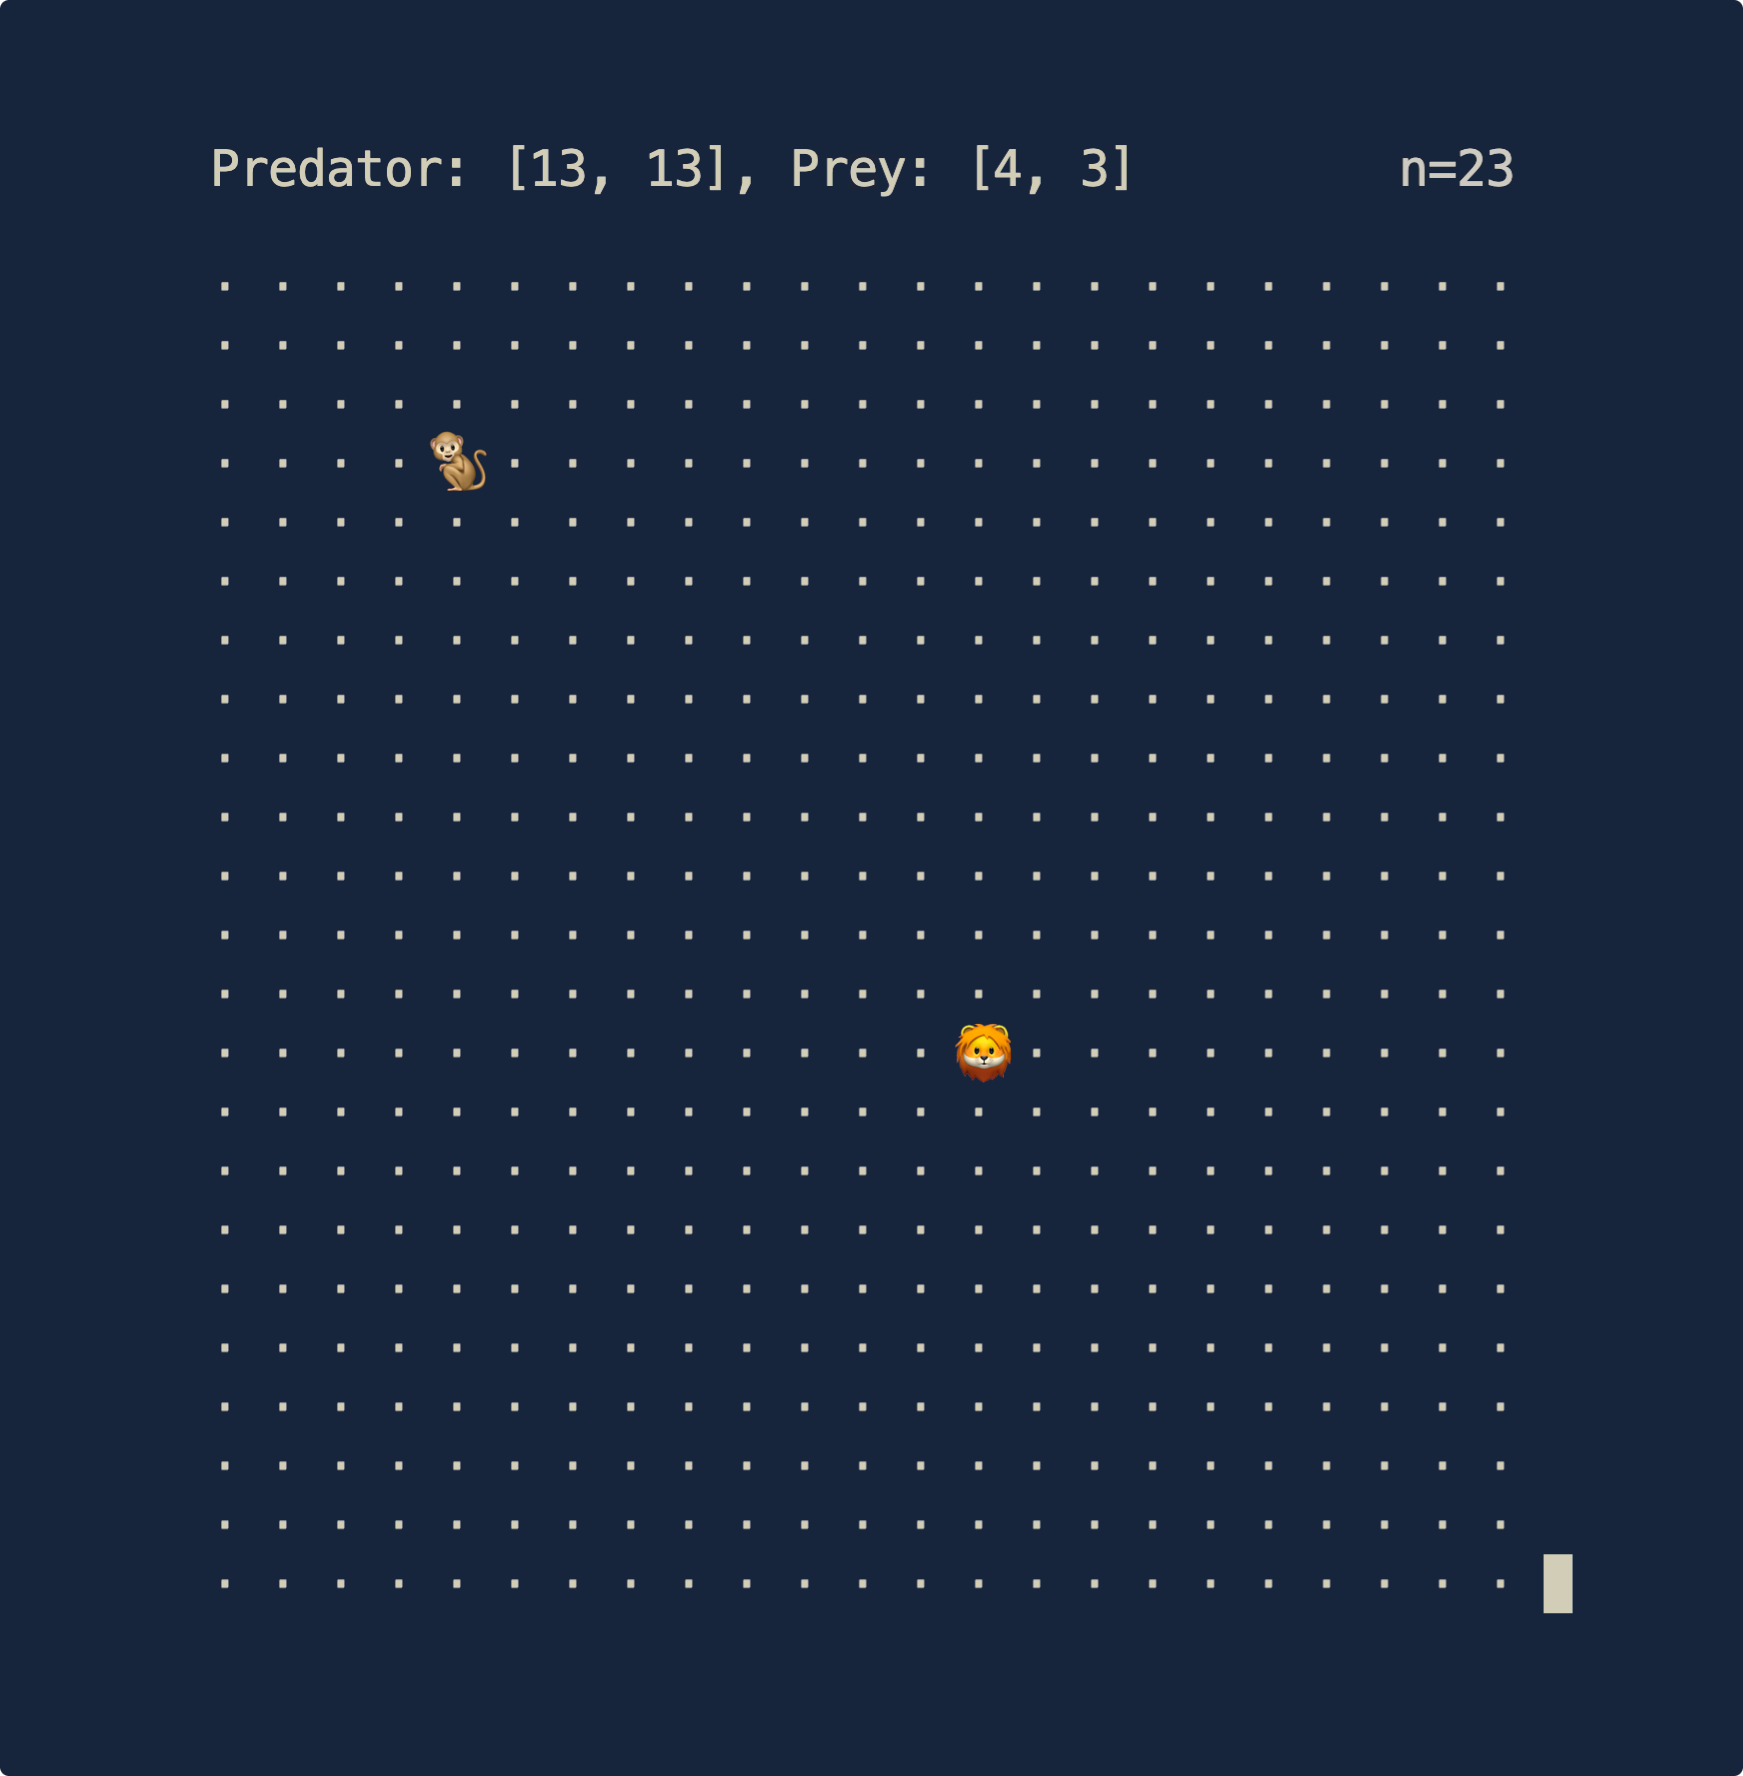
\includegraphics[width=0.6\textwidth]{lion-see-monke.png}
\end{figure}

\fontfamily{cmr}\selectfont
\color{white}-
\\[2pt]
\color{black}
\section*{Arbejdsfordeling}
Vi samarbejdede om alle opgaver, men uddelte løse \\ ansvarsområder til forskellige gruppemedlemmer.

s203775 var ansvarlig for: problem 1 og 3.a. \\
s194549 var ansvarlig for: problem 2 og hjælp på 3.b. \\
s204747 var ansvarlig for: 3.b. og hjælp på problem 3.a

\pagebreak

\section{Problem 1: Luhn algoritme / mod-10}
\subfile{problem_1}

\section{Problem 2: Interval Søgning}
\subfile{problem_2}

\section{Problem 3: Prey-Predator simulering}
\subfile{problem_3}

\pagebreak
\section{Bilag: Java klasser}
\label{appendix}
\subsection*{Problem 1, Java implementering}
\lstinputlisting{"../classes/NumberCheck.java"}
\subsection*{Problem 2, Java implementering}
\lstinputlisting{"../classes/IntervalSearch.java"}
\subsection*{Problem 3.a, Java implementering}
\lstinputlisting{"../classes/PredatorPray.java"}
\subsection*{Problem 3.b, Java implementering}
\lstinputlisting{"../classes/PredatorPrayTeleport.java"}
\subsection*{Problem 3: bonus, Java implementering}
\lstinputlisting{"../classes/PredatorVisualizer.java"}
\section{Bilag: Luhn / mod-10 implementering}
\label{app:Luhn}
\subfile{appendixLuhn}
\end{document}
